\chapter{Electronic Design}

\graphicspath{{./Figures/Electronic Design/}}

%figure of the electronic design
\begin{figure}[h]
	\centering
	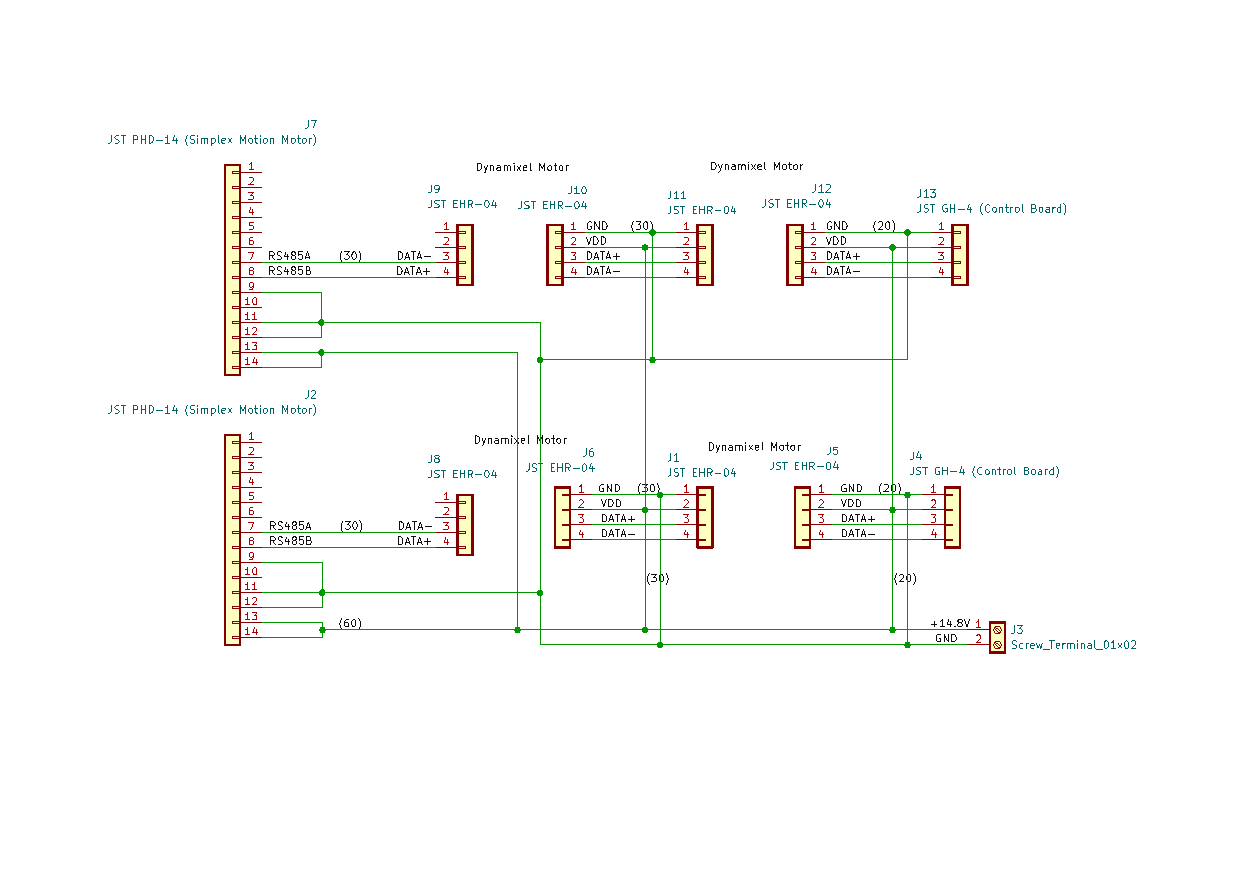
\includegraphics[width=1\linewidth]{Legged_TWIPR_Wiring_Tree}
	%\includegraphics[width=0.5\linewidth]{Figures/Mechanical Design/Conceptual_Design}
	\caption{Electronic Design}
	\label{fig:electronicdesign}
\end{figure}
\begin{itemize}
	\item Overview of the chapter's focus.
	\item Emphasize the importance of electronic design in the context of the overall project.
\end{itemize}


\section{Design Objectives and Constraints}
\begin{itemize}
	\item Clearly define the objectives and goals for the electronic design
	\item Discuss any constraints such as power requirements, size limitations.
\end{itemize}
\section{Component Selection}
\begin{itemize}
	\item Detail the selection process for key electronic components like microcontrollers, sensors, actuators, power supplies, etc.
	\item Rationale behind the choice of each component, focusing on specifications and performance requirements.
\end{itemize}
\section{Circuit Design}
\begin{itemize}
	\item Provide comprehensive information about the circuit design, including schematic diagrams.
	\item Explain the functionality and interaction of different circuit components.
	\item Discuss the design considerations for signal integrity, power distribution, and noise reduction.
\end{itemize}
\section{PCB (Printed Circuit Board) Design}
\begin{itemize}
	\item Describe the layout and design of any custom PCBs used in the project.
	\item Include information about PCB fabrication and assembly processes.
\end{itemize}
\section{Power Management}
\begin{itemize}
	\item Discuss how power is managed and distributed within the system.
	\item Include details on battery management, voltage regulation, and power efficiency considerations.
\end{itemize}